\documentclass{beamer}
\usepackage{amsmath}
\usepackage{amsfonts}
\usepackage{xeCJK}
\usepackage{tikz}
\usetikzlibrary{graphs}
\author{mapoet,付乃锋}
\institute{Shao}
\title{Introduce to Tikz}
\begin{document}
\begin{frame}{Slice 1}
\maketitle
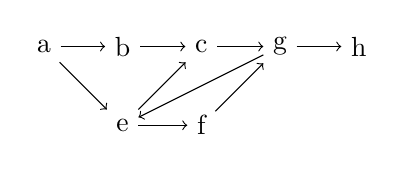
\begin{tikzpicture}
\graph{
	a -> {
		b -> c,
		e -> f
	} -> g ->
{ 
	e -> c,
	h
} 
};
\end{tikzpicture}
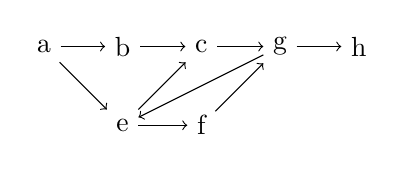
\begin{tikzpicture}
\graph{
	a -> {
		b -> c,
		e -> f
	} -> g ->
{ 
	e -> c,
	h
} 
};
\end{tikzpicture}
\end{frame}
\section{Rugger-kutta}
\begin{frame}
$$\frac{\partial Y}{\partial t}=F(t,X_t,Y_t)$$
$$\frac{d^n F(t,X_t,Y_t)}{d t^n}=F_n(t,X_t,Y_t)$$
$$F(t,X_t,Y_t)=F(t_0,X_{t_0},Y_{t_0})+\sum_{n=1}^{\infty}{\frac{F_n(t_0,X_{t_0},Y_{t_0})}{n!}(t-t_0)^n}$$
$$Y_t - Y_{t_0}=F(t_0,X_{t_0},Y_{t_0}){\delta t}$$

\end{frame}
\begin{frame}
$$\frac{\partial Y}{\partial X}=F(X,Y)$$
$$\frac{d^n F(X_t,Y_t)}{d t^n}=F_n(X_t,Y_t)$$
$$F(X_t,Y_t)=F(X_{t_0},Y_{t_0})+\sum_{n=1}^{\infty}{\frac{F_n(X_{t_0},Y_{t_0})}{n!}(t-t_0)^n}$$
$$Y_t - Y_{t_0}=F(X_{t_0},Y_{t_0}){\delta t}$$

\end{frame}
\section{Relativity}
\begin{frame}
$$G_{\mu \nu}+\Lambda g_{\mu \nu}=\frac{8 \pi G}{c^4}T_{\mu\nu}$$
$$G_{\mu \nu}=R_{\mu \nu}-\frac{1}{2}g^{\mu \nu}R_{\mu \nu}g_{\mu\nu}$$
$$\frac{d^2 x^{\lambda}}{d^2  \tau}+\Gamma^{\lambda}_{\mu \nu}\frac{d x^{\mu}}{d \tau}\frac{d x^{\nu}}{d  \tau}=0$$
$$\Box \phi=4 \pi T^{\mu \nu}[\eta_{\mu \nu}e^{-2\phi}+(e^{2\phi}+e^{-2\phi})\partial_{\mu}t\partial_{\nu}t],(1973)$$
\end{frame}
\begin{frame}
$$
\Delta f=[\frac{\partial^2}{\partial r^2}+\frac{N-1}{r}\frac{\partial}{\partial r}+\frac{1}{r^2}\Delta_{S^{N-1}}]f
$$
$$
\nabla_\ell V^m=\frac{\partial V^m}{\partial x^\ell}+\Gamma^m_{k \ell}V^k
$$
\end{frame}
\end{document}
